\documentclass[tikz,border=2pt]{standalone}
\usepackage{amsmath,amssymb}
\usepackage{pgfplots}
\pgfplotsset{compat=1.18}

\begin{document}
% Law of total expectation over the partition {A, A^c}: P(A) = 0.3 with E[Y | A] = 10 and
% P(A^c) = 0.7 with E[Y | A^c] = 2. Bar width = probability, height = conditional mean; the
% total area 3 + 1.4 = 4.4 is E[Y].
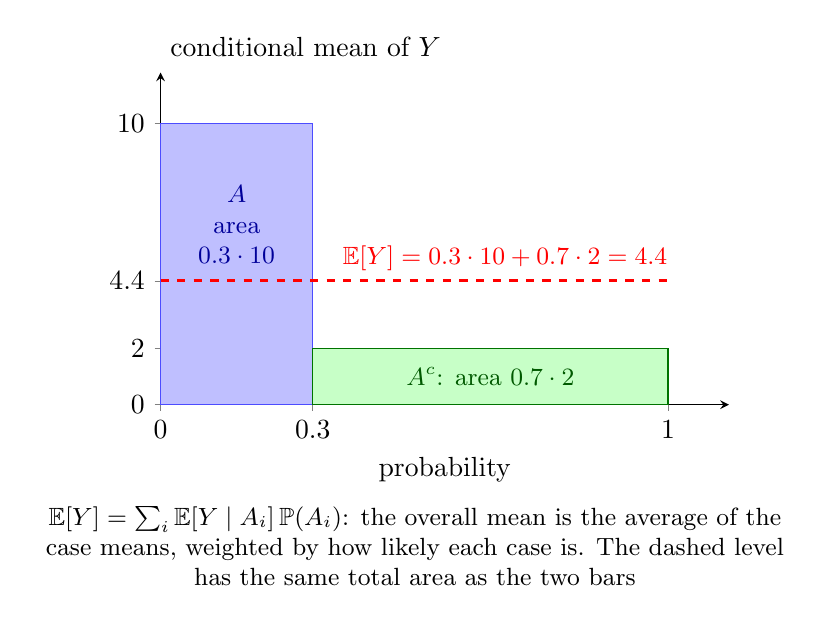
\begin{tikzpicture}
	\begin{axis}[
		axis lines=left, xmin=0, xmax=1.12, ymin=0, ymax=11.8,
		xtick={0,0.3,1}, ytick={0,2,4.4,10},
		xlabel={probability}, ylabel={conditional mean of $Y$}, ylabel style={rotate=-90, anchor=south west, at={(axis description cs:0,1.02)}},
		width=8.8cm, height=5.8cm, clip=false
		]
		\fill[blue!25] (axis cs:0,0) rectangle (axis cs:0.3,10);
		\draw[blue!70] (axis cs:0,0) rectangle (axis cs:0.3,10);
		\fill[green!22] (axis cs:0.3,0) rectangle (axis cs:1,2);
		\draw[green!45!black] (axis cs:0.3,0) rectangle (axis cs:1,2);
		\draw[red, dashed, very thick] (axis cs:0,4.4) -- (axis cs:1,4.4);
		\node[blue!60!black, font=\small, align=center] at (axis cs:0.15,6.4) {$A$\\ area\\ $0.3\cdot10$};
		\node[green!35!black, font=\small] at (axis cs:0.65,1) {$A^c$: area $0.7\cdot2$};
		\node[red, anchor=south west, font=\small] at (axis cs:0.34,4.4) {$\mathbb{E}[Y]=0.3\cdot10+0.7\cdot2=4.4$};
	\end{axis}
	\node[anchor=north, font=\small, align=flush center, text width=9.6cm] at ([yshift=-2pt]current axis.outer south) {$\mathbb{E}[Y]=\sum_i\mathbb{E}[Y\mid A_i]\,\mathbb{P}(A_i)$: the overall mean is the average of the case means, weighted by how likely each case is. The dashed level has the same total area as the two bars};
\end{tikzpicture}
\end{document}
